\documentclass{scrartcl}
\usepackage{amsmath,amsfonts,amsthm,bm,graphicx}
\usepackage{tikz,pgfplots}
\usepackage{listings}
\usepackage{stmaryrd}
\usepackage{xcolor}
\usepackage{fdsymbol}
\usepackage{rotating}
\usepackage{listings}
\usepackage{hyperref}

\pgfplotsset{width=15cm,compat=1.18}
\allowdisplaybreaks
\setlength{\parindent}{0pt}

\title{Assignment 3: Fourier Transformation in Matlab}
\subtitle{Angewandte Modellierung 25}
\author{Carl Colmant}
\date{\today}
\begin{document}
\maketitle
\newpage
\section*{Exercize 1. Modellierung von Sinussignalen}
Zu erst habe ich die Blöcke wie in der Aufgabe beschrieben erstellt (meine letzte Ziffer der matrikelnr. ist 2).\\
Dabei entstehen folgende Spektren:\\
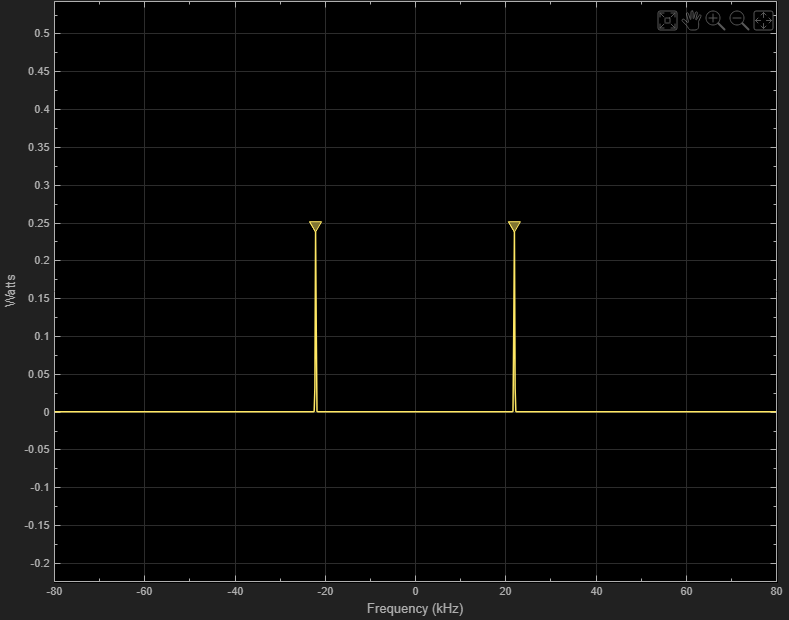
\includegraphics[scale=0.5]{spectrum.png} \\
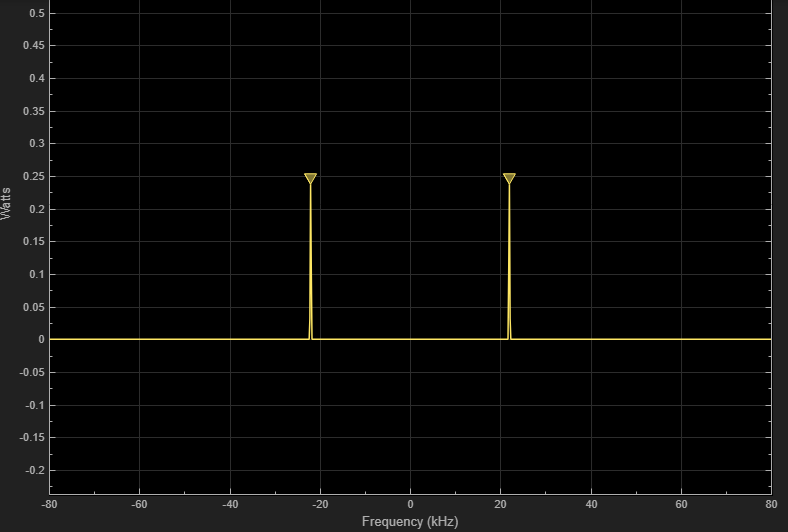
\includegraphics[scale=0.5]{spectrum1.png} \\
Und das Spectrum der Summe der Signale:\\
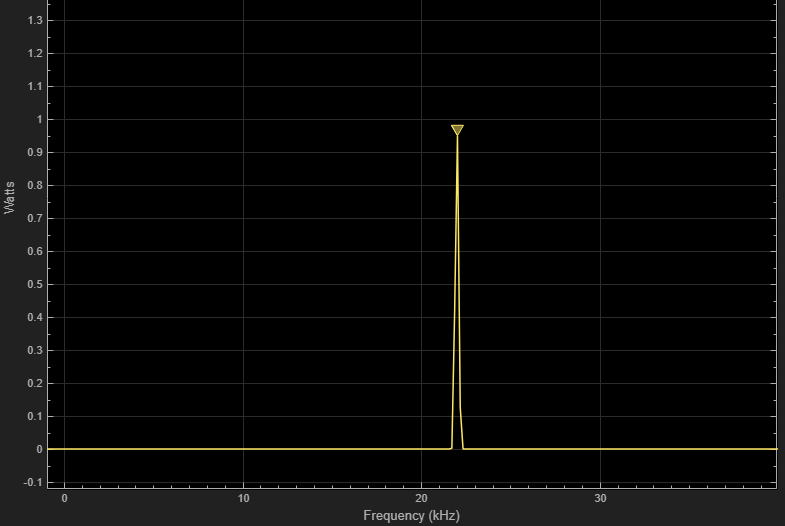
\includegraphics[scale=0.5]{spectrumAdd.png} \\

Die beiden Sinus funktionen haben die Frequenz 22000Hz die erste wird um $\frac{\pi}{2}$ verschoben heißt also $sin(22000 \cdot t + \frac{\pi}{2})$ und die zweite ist $sin(22000 \cdot t)$. Weil die beiden Signale die gleiche Frequenz haben, bekommen wir im Spectrum Analyzer den selben Peak bei 22000Hz und -22000Hz.\\ 
Die zweite Sinus Funktion wird vor dem Addieren noch mit j multipliziert. Das heißt wir addieren $cos(22000t) + j*sin(22000t) = e^{j*22000t}$ und das ist die Darstellung der komplexen Exponentialfunktion. Die nur eine Spectrallinie hat bei 22000Hz.\\

Das kann auch in der Simulation gesehen werden.\\

\subsection*{Frequenz Veränderung}
Die Frequenz der Sinus Signale wird in Block Sine Wave 1 auf $2\pi * 3000$ verringert. Nun haben wir keine gleichen Frequenzen der beiden Signale das heißt es entsteht ein überlagertes komplexes Signal, mit 2 SPectral linien.\\

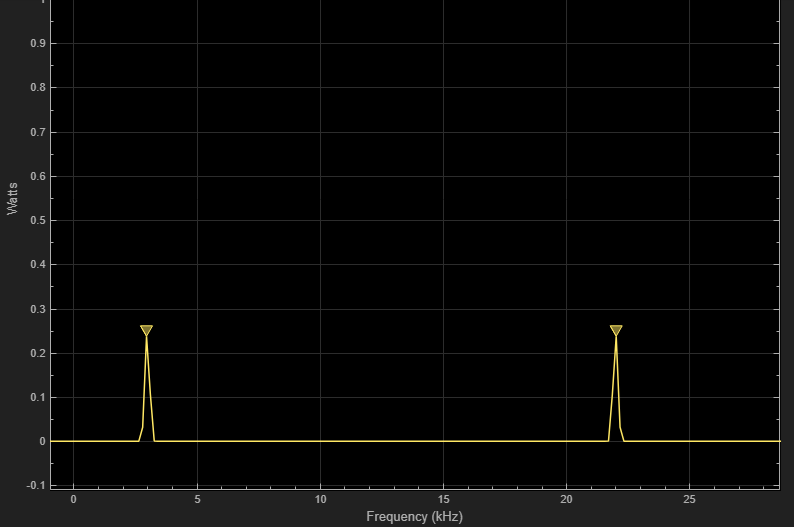
\includegraphics[scale=0.5]{spectrumAdd2.png} \\

\subsection*{Phasen Verschiebung}
Wenn man die Phase im zweiten Sine wave Block auf $4$ setzt ergibt sich kein Unterschied im Spectrum. Das liegt daran das sich die Phase nicht auf die Frequenz auswirkt.\\

\section*{Exercize 2: Analyse von puls Generator Spektren}

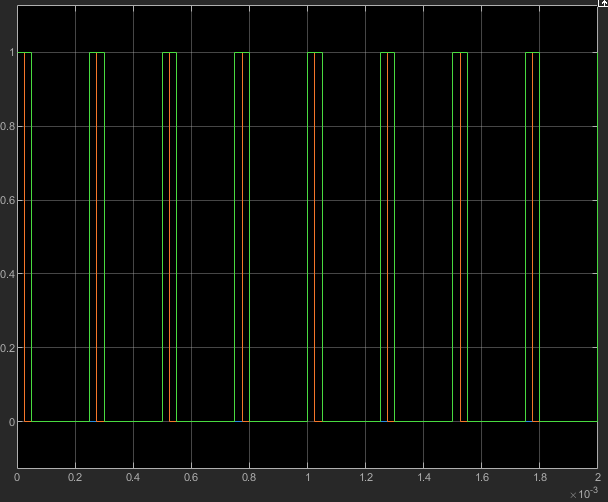
\includegraphics[scale=0.5]{PulseScope.png}

Wenn man sich den Scope ansieht sieht man das der dritte und vierte Puls Block die doppelte Frequenz hat wie der erste und zweite. Nun ist die Pulse width im ersten block 5\% und im zweiten 10\%. Der dritte block hat die doppelte Pulse width wie der erste Block also auch 10\% und damit die selbe width. Der vierte Block hat die doppelte width wie der zweite Block (20\%) und damit die selbe width. Das liegt daran dass die breite des Puls mit der Periode wächst und der Dritte und vierte Block die hälfte der Periodenzeit haben wie der erste und zweite Block. Die Frequenz unterschiede sind auch auf die unterschiedlichen Periodenzeiten zurückzuführen($freq = \frac1{periode}$) \\ 

Der Intervall zwischen zwei Spektrallinien sollte nach der Formel 2kHz sein, das lässt sich so ungefähr auch im Spectrum Analyzer ablesen mithilfe von dem Data cursor.\\ %Das ist noch nicht ganz richtig abhängig von der Frequenz(?) verändert sich die INtervall größe.\\
Der erste Nullpunkt des Pulses ist abhängig von der Pulse width und der Periodenzeit. So kleiner die Perioden Zeit desto größer die Puls Größe(also desto größer der Nullpunkt), genauso beeinflusst auch die Pulse width die Pulse Größe so kleiner sie ist desto später kommt der Nullpunkt.\\

\end{document}